\chapter{Research Methodology}
\label{ch:methodology}


\section{Research Design}

This is a retrospective, observational prediction-modelling study on
de-identified critical-care data. The original protocol (\S\S1--12 of
\texttt{00\_preregistration.md}) specified the research question, the six
hypotheses, the label variants, model classes, validation splits, metrics and
decision thresholds before any of the modelling reported here. The uncertainty
and multiplicity procedures were added after the initial analyses as Protocol
Amendment 1 and are described separately (Section~\ref{sec:inference_status}).
Reporting follows TRIPOD+AI \cite{collins2024tripodai} and PROBAST+AI
\cite{moons2025probastai}. The design treats the label definition, the timing
of prediction relative to treatment, the validation split and the evaluation
metric as study variables alongside the model. Implementation and dependency
details are given in Chapter~\ref{ch:design} and Appendix~\ref{app:repro}.

The design decisions were informed by the structured narrative search
described in Section~\ref{sec:search_strategy}. The search was not a
systematic review, and novelty claims are interpreted within the limits stated
there and in Section~\ref{sec:limitations}.


\section{Data Sources}
\label{sec:data}

\subsection{Development Data: MIMIC-IV v3.1}

The development dataset is MIMIC-IV v3.1
\cite{johnson2023mimiciv,johnson2023mimiciv_scidata,pollard2026physionet}, a
de-identified critical-care database from Beth Israel Deaconess Medical Center
(BIDMC), Boston, accessed through PhysioNet credentialing. Eight source tables
were used (Table~\ref{tab:data_sources}).

\begin{table}[H]
    \centering
    \begin{tabular}{lr}
        \toprule
        \textbf{Table}     & \textbf{Size (MB)} \\
        \midrule
        admissions         & 19.9               \\
        patients           & 2.8                \\
        icustays           & 3.3                \\
        chartevents        & 3,502.6            \\
        labevents          & 2,593.0            \\
        prescriptions      & 606.7              \\
        microbiologyevents & 117.2              \\
        inputevents        & 401.3              \\
        \bottomrule
    \end{tabular}
    \caption{MIMIC-IV v3.1 source tables used in this study, with compressed
    file sizes.}
    \label{tab:data_sources}
\end{table}

\subsection{External Validation Data: eICU-CRD v2.0}

External validation uses eICU-CRD v2.0 \cite{pollard2018eicu}, a multicentre
database from more than 200 US ICUs, recorded in different electronic health
record systems and covering a broader range of hospitals than the single-centre
MIMIC-IV. The frozen MIMIC-IV models are applied to harmonised features
without retraining.

\subsubsection{Transporting the label as well as the model}
\label{sec:label_transport}

Sepsis-3 onset is defined on documentation (an antibiotic order, a
microbiology culture) whose recording conventions differ between databases
more than physiology does, so the label has to be reconstructed in eICU-CRD
rather than transported with the model. Three properties of eICU-CRD govern
its construction.

\textbf{Drugs are recorded across two tables.} eICU-CRD has no item
dictionary; drugs are free-text names split between \texttt{medication}
(orders) and \texttt{infusionDrug} (continuous infusions), and vasopressors and
much of the intravenous antibiotic exposure appear only in the latter.
Antibiotic exposure is the union of both tables, and vasopressor exposure is
taken from \texttt{infusionDrug} so that the SOFA cardiovascular component is
not fixed at its no-vasopressor value.

\textbf{Microbiology availability limits the Sepsis-3 label.} The suspicion
anchor requires a culture, and \texttt{microLab} covers \pcExtNMicroStays{} of
\pcExtNCohortStays{} unit stays (\pcExtMicroCoverage\%). Culture availability
is necessary but not sufficient for assigning the label: both limbs are
documented for \pcExtNBothLimbStays{} stays (\pcExtBothLimbCoverage\%), and
fewer remain once each variant's windows and organ-dysfunction criterion are
applied (Section~\ref{sec:external_coverage}). The primary external analysis
is therefore restricted to the microbiology-covered sub-cohort, in which an
onset is observable, and its event rate is compared with MIMIC-IV's on that
basis.

\textbf{The organ-dysfunction criterion is a rise, not a level.} Onset is
gated on a SOFA increase of at least two points over a baseline, evaluated
inside each variant's own window and against its own baseline (admission for
Variants A and B, rolling 24-hour for Variant C), as in the development
cohort. An absolute SOFA threshold would be a different criterion, and because
missing components are scored at assumed-normal values it would reject stays
for incomplete documentation rather than intact organ function, biasing
towards the null in a database with sparser laboratory coverage than
MIMIC-IV.

Each label variant retains its own antibiotic--culture windows and SOFA
baseline in eICU-CRD, so the external label sets differ from one another as
they do internally. Two further external analyses are reported separately and
never pooled with the primary one. An \textbf{antibiotic-only} analysis relaxes
the culture requirement across the full cohort to measure how much of the
event count that requirement removes; its target is not Sepsis-3. Under
Protocol Amendment 9 (post-hoc), the frozen Variant D models
(Section~\ref{sec:alt_labels}) are applied to the full cohort, which Variant
D's culture-free onset rule permits. eICU-CRD's periodic vital-sign table
carries no Glasgow Coma Scale, so the external SOFA rise for Variant D rests on
five components rather than MIMIC-IV's six (Section~\ref{sec:external_altlabel}).


\section{Ethical Considerations}
\label{sec:ethics}

This study uses two de-identified critical-care databases distributed through
PhysioNet. Neither contains protected health information as defined under
HIPAA, and no re-identification was attempted.

\textbf{MIMIC-IV v3.1} is distributed by the MIT Laboratory for Computational
Physiology via PhysioNet \cite{johnson2023mimiciv}. Access requires completion
of the Collaborative Institutional Training Initiative (CITI) ``Data or
Specimens Only Research'' course and signing a PhysioNet Credentialed Data Use
Agreement (DUA). The DUA prohibits re-identification and restricts data sharing
to credentialed collaborators. The author completed CITI training and executed
the DUA before any data access; credentials are on file with PhysioNet.
\textbf{eICU-CRD v2.0} \cite{pollard2018eicu} is distributed under the same
PhysioNet credentialing framework and DUA terms.

Both databases are distributed as de-identified research datasets under the
institutional approvals obtained by their custodians and PhysioNet's
credentialing requirements. This study is a secondary analysis only, with no
patient contact, intervention or attempt at re-identification, and the terms
of the applicable data use agreements were followed throughout.


\section{Cohort Construction}
\label{sec:cohort}

The base cohort is built by applying three inclusion criteria uniformly across
all label variants:

\begin{itemize}
    \item Age $\geq 18$ at ICU admission.
    \item First ICU stay per patient only (to prevent within-patient correlation).
    \item ICU length of stay $\geq 4$ hours (to permit hourly feature
    construction and at least one prediction).
\end{itemize}

The resulting cohort contains \textbf{\pcNStays{} stays} in MIMIC-IV.
Figure~\ref{fig:consort} shows the patient flow through each exclusion step.

\begin{figure}[H]
    \centering
\adjustbox{max width=\textwidth}{%
    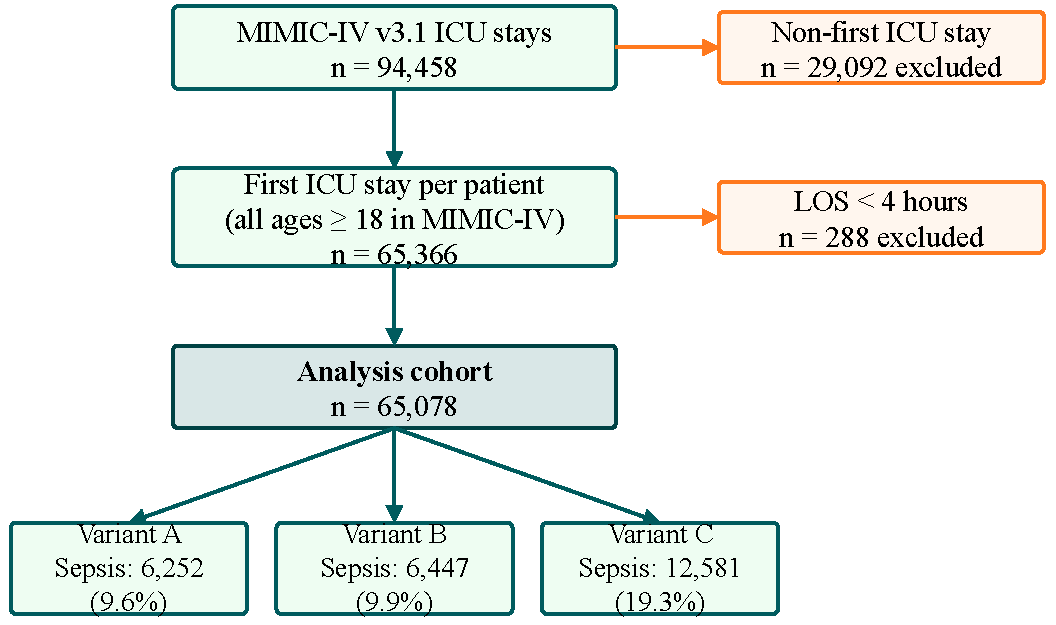
\includegraphics[width=\textwidth]{figures-img/fig3.1_consort.pdf}}
    \caption{CONSORT-style patient flow diagram. All \pcConsortNFinal{} stays enter
    all three label variants; only the sepsis outcome differs. Every count is
    generated from \texttt{02\_cohort\_flow}, written by script
    \texttt{02\_cohort\_labels.Rmd}. The age criterion is applied first and
    excludes \pcConsortNExclAge{} stays, which is why it appears as an
    annotation rather than as an exclusion box: MIMIC-IV's ICU module records
    adult admissions only. The filter is nevertheless run and its count
    generated. Sepsis counts are \textbf{cohort-wide},
    at any hour of the stay; the subset falling inside the 72-hour modelling
    horizon, which is what the models are trained and evaluated on, is reported
    in the results chapter.}
    \label{fig:consort}
\end{figure}


\section{Outcome Definition: Three Sepsis-3 Label Variants}
\label{sec:label_variants}

Following Cohen et al.\ \cite{cohen2024subtle} and Johnson et al.\
\cite{johnson2018comparative}, three operationalisations of Sepsis-3 were
evaluated. All three are plausible operationalisations of the same consensus
definition \cite{singer2016sepsis3}; they differ in their antibiotic--culture
windows and SOFA baselines (Table~\ref{tab:label_variants}).

\begin{table}[H]
    \centering\small
    \adjustbox{max width=\textwidth}{%
    \begin{tabular}{llccccc}
        \toprule
        \textbf{ID} & \textbf{Name} & \textbf{ABX$\to$cx} & \textbf{cx$\to$ABX}
        & \textbf{SOFA$-$} & \textbf{SOFA$+$} & \textbf{Baseline} \\
        \midrule
        A & Narrow      & 24\,h & 24\,h & 24\,h & 12\,h & Admission     \\
        B & Seymour-Std & 72\,h & 24\,h & 48\,h & 24\,h & Admission     \\
        C & Liberal     & 72\,h & 72\,h & 48\,h & 24\,h & Rolling 24\,h \\
        \bottomrule
    \end{tabular}}
    \caption{Three pre-registered Sepsis-3 label variants. ABX = antibiotic;
    cx = culture; SOFA$-$/SOFA$+$ = hours before/after suspicion time in which
    a SOFA rise of $\geq 2$ must be observed. Baseline = SOFA reference value.}
    \label{tab:label_variants}
\end{table}

In all three variants, a patient has sepsis if there is suspected infection
(antibiotic order paired with a culture within the specified windows) and the
SOFA score increases by at least 2 points. Surveillance cultures (e.g.\ MRSA
screens) are excluded.

Variant B (Seymour-Standard) is the \textbf{primary analysis}. Variants A and C
are pre-specified sensitivity analyses for the variance decomposition.


\section{Beyond Sepsis-3: An Anchor-Independent Label}
\label{sec:alt_labels}

Variants A--C share a culture-plus-antibiotic suspicion anchor, which records a
clinician's decision to treat. Any change to the antibiotic--culture windows
therefore moves the onsets, so part of the label-variant spread follows from
the definition itself (\textbf{definitional} variation). Whether a label that
does not use treatment timing selects different patients, at different hours,
with different predictability is an \textbf{empirical} question, and it cannot
be assessed within a family of labels that share the anchor.

Protocol Amendment 2 (post-hoc) therefore splits the Sepsis-3 conjunction of
\emph{suspected infection} and \emph{acute organ dysfunction} and labels each
component separately (Table~\ref{tab:alt_label_variants}): Variant E retains
the suspicion anchor without requiring organ dysfunction, and Variant D retains
organ dysfunction without using treatment timestamps.

\begin{table}[H]
    \centering\small
    \begin{tabular}{llccp{3.1cm}}
        \toprule
        \textbf{ID} & \textbf{Name} & \textbf{Suspicion anchor}
        & \textbf{Organ dysf.} & \textbf{Uses treatment timing?} \\
        \midrule
        B & Seymour-Std    & required     & required     & \raggedright membership and timing\tabularnewline
        E & Anchor-Only    & required     & not required & \raggedright yes\tabularnewline
        D & Deterioration  & not required & required     & \raggedright \textbf{no}\tabularnewline
        F & Sepsis-3 Early & required     & required     & \raggedright membership only\tabularnewline
        \bottomrule
    \end{tabular}
    \caption{The two limbs of the Sepsis-3 conjunction labelled separately
    (Variants E and D, Protocol Amendment 2), and the standard onset timing
    applied to the intact conjunction (Variant F, Protocol Amendment 4).
    Variant F has Variant B's membership and differs only in when the onset is
    placed.}
    \label{tab:alt_label_variants}
\end{table}

\textbf{Variant E (Anchor-Only)} takes onset to be the suspicion time itself,
using Variant B's windows, with no organ-dysfunction requirement, so its label
records clinician behaviour only. The share of Variant B's above-chance
discrimination that Variant E reproduces,
\begin{equation}
    \phi_{\text{anchor}}
    = \frac{\mathrm{AUROC}_E - 0.5}{\mathrm{AUROC}_B - 0.5},
    \label{eq:anchor_fraction}
\end{equation}
is reported as the \textbf{anchor-attributable fraction}.

\textbf{Variant D (Deterioration)} takes onset to be the first hour after hour~1
at which a \emph{physiology-only} SOFA score rises at least 2 points above the
patient's admission baseline (the mean of each component over hours 0--3). The
vasopressor and catecholamine terms are withheld, so the cardiovascular
component is scored from mean arterial pressure alone, and no antibiotic order,
culture draw or drug administration enters the definition. Variants D and E are
fitted with the same model specification, feature set and temporal split as
Variant B, so only the label changes.

Here, ``anchor-independent'' means that antibiotic, culture and vasopressor
timestamps do not determine label membership or onset. It does not imply
independence from clinical care or documentation: Variant D is built from
measurements that exist because they were ordered, on patients whose
physiology already reflects any treatment received.

The PhysioNet/CinC 2019 operationalisation \cite{reyna2020utility} was
considered as the anchor-independent label and rejected for that purpose: it
sets onset to $\min(t_{\text{susp}}, t_{\text{SOFA}})$ with the same
culture-plus-antibiotic trigger, so membership remains anchored to treatment.
SEP-1 and the CDC Adult Sepsis Event \cite{dutta2026performance} are excluded
for the same reason, since both are defined on antibiotic days.

Variants D and E are used only for exploratory attribution. Variant~E
represents the treatment anchor rather than sepsis, so its AUROC is not a
sepsis result. Variant~D is an unvalidated deterioration label derived from
recorded physiology, and five of its six SOFA components are also model
inputs, so its discrimination is partly self-fulfilling and its \emph{level}
is not comparable with Variant~B's. The principal comparisons are therefore
onset agreement (Cohen's $\kappa$) and median onset shift
(Section~\ref{sec:label_anchor_results}).

\subsection{Standard Onset Timing (Variant F, Protocol Amendment 4)}
\label{sec:variant_f}

Variants A--C assign onset $= t_{\text{susp}}$ whenever the SOFA criterion is
satisfied anywhere in the evaluation window, so the SOFA criterion gates
membership and contributes no timing information. Under this rule no onset can
precede the first antibiotic or culture, and the pre-treatment window of H3 is
empty by construction (Proposition~\ref{prop:h3} in
Chapter~\ref{ch:evaluation}). Seymour et al.\ \cite{seymour2016assessment} and
the PhysioNet/CinC 2019 Challenge \cite{reyna2020utility} instead assign
\begin{equation}
    t_{\text{onset}} = \min\bigl(t_{\text{susp}},\, t_{\text{SOFA}}\bigr),
    \label{eq:early_onset}
\end{equation}
with $t_{\text{SOFA}}$ the first hour in the evaluation window at which the
$\geq 2$-point rise over the admission baseline is present.

Protocol Amendment 4 introduced Variant F after this limitation of the
pre-registered onset rule was identified and before Variant F was fitted.
\textbf{Variant F (Sepsis-3 Early-Onset)} retains Variant B's suspicion
windows, SOFA threshold, evaluation window and baseline, and assigns onset by
Equation~\eqref{eq:early_onset}. The two variants therefore label the same
stays cohort-wide, and Variant F's onset is never later than Variant B's.

Here $t_{\text{SOFA}}$ uses the \emph{full} SOFA score, vasopressor components
included, as Seymour et al.\ specify, so an onset placed by the cardiovascular
component is free of the antibiotic--culture anchor but not of treatment in
general; Variant D remains the anchor-independent comparison. Because
stay-level membership is identical, the informative agreement statistic for
Variant F is the onset \emph{shift} rather than the overlap. Earlier onset
assignment can also move events into the 72-hour modelling horizon when
Variant B's suspicion time falls later, so within the horizon Variant F may
contain more events than Variant B despite identical cohort-wide membership
(Section~\ref{sec:pretreatment_label}).

Variants D, E and F are post-hoc and are excluded from the pre-registered
variant set: they take no part in H1 or the variance decomposition, which are
computed from unchanged inputs. Their contrasts against Variant B form
exploratory family E3, corrected by Benjamini--Hochberg.


\section{Prediction Framing}
\label{sec:framing}

Following Lauritsen et al.\ \cite{lauritsen2021framing} and Reyna et al.\
\cite{reyna2020utility}, the prediction problem is framed as follows:

\begin{itemize}
    \item \textbf{Observation window:} Expanding from ICU admission, uses all
    data available up to the current hour.
    \item \textbf{Estimand:} the \emph{cause-specific discrete-time hazard} of
    sepsis onset in the current hour, conditional on the stay being at risk at
    the start of it, $\Pr(\text{onset at hour } t \mid \text{at risk at } t,
    \mathbf{x}_t)$, with discharge and death as competing causes.
    \item \textbf{Prediction frequency:} Every hour.
    \item \textbf{Start time:} 1 hour after ICU admission.
    \item \textbf{End time:} 72 hours after ICU admission (right-censored).
    \item \textbf{Alerting window:} 6 hours. An alert counts as timely if it is
    issued in the six hours up to onset.
\end{itemize}

\paragraph{Estimand and scoring target.} AUROC, AUPRC and calibration are
computed on this hazard against an indicator that is one at the onset hour and
zero at every other at-risk hour. They therefore evaluate onset-hour
detection, not a binary ``onset within six hours'' target. The six-hour window
is used only for the Utility Score, per-patient detection and lead-time
metrics (Section~\ref{sec:metrics}).

Predictors and outcomes are aggregated to the same elapsed hour, so
measurements recorded after the exact onset timestamp but within the same
hourly bin can contribute to the onset-hour prediction. Reported
discrimination should therefore be read as detection at the recorded onset
hour, not as demonstrated advance warning (Limitation~\ref{lim:current_hour}).

The hazard formulation was retained because cumulative risk over a horizon
depends on both the sepsis and the competing-event hazards over that horizon.
It does not yield a single measure of six-hour discrimination, a limitation
recorded in Section~\ref{sec:limitations}. The alerting window and the utility
scoring rule are adapted from the PhysioNet/CinC 2019 Challenge
\cite{reyna2020utility} rather than reproduced from it
(Section~\ref{sec:metrics}), and the estimand differs from the Challenge's,
which scored a binary label defined over the window itself.


\section{Person-Hour Table and Competing Events}
\label{sec:person_hours}

Each patient stay is expanded into a table with one row per person-hour at
risk. Following Heyard et al.\ \cite{heyard2019dynamic}, each hour is
assigned one of four outcomes:

\begin{itemize}
    \item 0: No event in this hour; the stay remains at risk
    \item 1: Sepsis onset (the event of interest)
    \item 2: Discharged alive without sepsis (competing event)
    \item 3: Died without sepsis (competing event)
\end{itemize}

Discharge and death are treated as competing events rather than as
non-informative censoring, because both remove a stay from the risk set and
may be associated with sepsis risk.


\section{Feature Construction}
\label{sec:features}

Features are extracted at each person-hour from chartevents, labevents and
inputevents. The feature set includes:

\begin{enumerate}
    \item \textbf{Vital signs}, 6 (last value carried forward per hour): heart
    rate, respiratory rate, SpO$_2$, MAP (invasive or noninvasive), temperature
    ($^\circ$C), GCS total.
    \item \textbf{Laboratory values}, 5 (last value carried forward): lactate,
    creatinine, total bilirubin, platelet count, WBC.
    \item \textbf{Vasopressor indicators}, 2: any vasopressor (yes/no); any
    norepinephrine or epinephrine (yes/no).
    \item \textbf{Six-hour trends}, 3: rolling slopes for heart rate,
    respiratory rate and MAP.
    \item \textbf{Missingness indicators}, 6: whether each of lactate,
    creatinine, bilirubin, platelets, white cells and a blood gas
    (P/F ratio) was ordered in the current hour, one flag per test.
\end{enumerate}

Temperature in Fahrenheit is converted to Celsius. FiO$_2$ values above 1.0
(percentage format) are divided by 100.

The P/F ratio is used in the SOFA respiratory component of the label but is
not a continuous predictor, because it is recorded for a minority of
person-hours and its forward-filled value reflects ventilation practice more
than the current hour; only its current-hour measurement indicator is
included. No lactate slope is calculated, because lactate is not sampled
densely enough to support a stable six-hour trend.

The declared set therefore holds \textbf{22 covariates}, and the fitted model
carries \textbf{29 terms per outcome} once the six-column natural-spline
baseline in elapsed hours and the intercept are counted. The feature vector is
defined centrally in \texttt{config.R}, and the model-fitting and transport
stages terminate with an error if a declared predictor is absent
(Chapter~\ref{ch:design}).


\section{Model Classes}
\label{sec:models}

\subsection[Primary Model: Dynamic Discrete-Time Competing-Risks Hazard Model]%
{Primary Model: Dynamic Discrete-Time Compet\-ing-Risks Hazard Model}
\label{sec:primary_model_spec}

The primary model is a multinomial pooled logistic regression over person-hours,
following D'Agostino et al.\ \cite{dagostino1990pooled} and Heyard et al.\
\cite{heyard2019dynamic}:

\begin{equation}
    \lambda_r(t \mid \mathbf{X}_{it}) =
    \frac{\exp\!\bigl(\alpha_r(t) + \boldsymbol{\beta}_r^\top \mathbf{X}_{it}\bigr)}
    {1 + \sum_{s} \exp\!\bigl(\alpha_s(t) + \boldsymbol{\beta}_s^\top \mathbf{X}_{it}\bigr)}
    \label{eq:primary_model}
\end{equation}

where $r \in \{1=\text{sepsis},\, 2=\text{discharge},\, 3=\text{death}\}$.
The baseline hazard $\alpha_r(t)$ uses a restricted natural cubic spline with
5 knots, placed at quantiles of training-set hour within each variant.

The model estimates the hazard of sepsis at every hour. With short intervals
and low interval-specific event probabilities, pooled logistic regression
closely approximates time-dependent Cox regression
\cite{dagostino1990pooled}, while permitting explicit modelling of competing
outcomes and requiring no proportional-hazards assumption.

\paragraph{Identification and penalisation.}
The unpenalised version of Equation~\eqref{eq:primary_model} is
\textbf{completely separated} under every label variant: under iteratively
reweighted least squares run to a tight tolerance, the whole coefficient vector
diverges together, with $|\beta|$ of order $10^{15}$, although the design
matrix is full rank. The optimiser nevertheless reports success:
\texttt{nnet::multinom} returns \texttt{convergence = 0}, which records only
that its stopping rule fired, not that a finite maximiser exists. A fixed ridge
penalty of $\lambda = 10^{-4}$ is therefore applied to obtain finite, stable
penalised estimates. The value is \textbf{not tuned}: across a 20-point ridge
path the temporal-test AUROC varies by less than 0.02 for every variant.
Coefficient comparisons across label variants (H2, Section~\ref{sec:h2}) refer
to the penalised estimates; without penalisation, a fit could stop at an
arbitrary point under one label and a different one under another, producing
an apparent label effect.

\paragraph{Coefficient uncertainty.}
Coefficient standard errors use a sandwich covariance clustered on the stay
(implementation in Chapter~\ref{ch:design}). Because the model is
ridge-penalised, these are standard errors of the \emph{penalised} estimator,
described as a ridge-regularised sandwich throughout. They do not provide
uncertainty for H2's count of unstable covariates, which is a threshold rule
applied across three separate fits, so H2 remains a descriptive count
(Section~\ref{sec:h2}).

\textbf{Protocol Amendment 7} (post-hoc, \S21 of
\texttt{00\_preregistration.md}) adds a diagnostic beside that count: for each
flagged covariate, the difference between its two extreme estimates is
divided by the pooled standard error of those two
(Section~\ref{sec:h2_uncertainty}). The ratio is reported alongside the
pre-registered count, never in place of it. It is not a test: the three fits
share stays, so the differenced estimates are correlated and a pooled standard
error assuming independence is conservative by an unquantified amount; it
carries no $p$-value and enters no corrected family. Every interval on a
performance quantity comes from the stay-level cluster bootstrap of
Section~\ref{sec:inference}, and the analytic covariance enters no hypothesis
verdict.

\subsection{Comparator: Gradient-Boosted Trees (GBT)}
\label{sec:gbt_spec}

A gradient-boosted tree (GBT) model is fitted with XGBoost for each label
variant and split, on the same 22 covariates as the primary model. Its
settings were fixed in advance and are applied identically to every variant,
split and feature arm: logistic objective, area under the precision-recall
curve as the evaluation metric, maximum depth 6, learning rate 0.05, row and
column subsampling at 0.8, minimum child weight 5, and positive-class
weighting by the observed class ratio. No hyperparameter search was conducted
for either the GBT or the primary model, which keeps the search budget equal
across the H6 comparison but may place the GBT below its attainable
performance (Chapter~\ref{ch:discussion}).

The number of boosting rounds is chosen by early stopping on a holdout drawn
from the \emph{training} rows: 15 per cent of training stays are held out, the
model is fitted on the remainder, and boosting stops after 30 rounds without
improvement on the holdout. The holdout is split by stay, because each stay
contributes roughly forty-five correlated person-hours and a row-level split
would place the same patient on both sides. The test set is never used to
select the number of rounds (Protocol Amendment 8).

\subsection{Comparator: Cox Proportional-Hazards Model}
\label{sec:cox_spec}

A Cox proportional-hazards model is included as a conventional survival-model
comparator. The pre-registration calls it the \emph{static} comparator, which
refers to its coefficients rather than its inputs: it is a Cox model with
time-varying covariates and time-constant coefficients. It is fitted on the
same training person-hours as every other comparator, in counting-process
form: each hour contributes the interval $(t,\, t+1]$ with that hour's event
indicator, so its covariates are the same hourly, forward-filled values the
primary model sees. Each covariate has one time-constant log hazard ratio, the
baseline hazard is left unspecified, and no interaction with elapsed time is
estimated; Section~\ref{sec:schoenfeld} tests this assumption with Schoenfeld
residuals.

The specification otherwise differs from the primary model:

\begin{itemize}
    \item \textbf{Covariates.} Twelve of the primary model's twenty-two: heart
    rate, respiratory rate, oxygen saturation, mean arterial pressure,
    temperature, Glasgow Coma Scale, lactate, creatinine, total bilirubin,
    platelets, white cell count, and any vasopressor exposure. The three
    six-hour slope features, the second vasopressor indicator and the six
    order (\emph{measured}) indicators are \emph{not} included.
    \item \textbf{Time origin and risk set.} Elapsed hours since ICU admission,
    the same clock the primary model splines; a stay is at risk from hour one
    until onset, discharge, death or hour 72.
    \item \textbf{Event and competing events.} The event is sepsis onset in the
    hour. Unlike the multinomial primary model, the Cox specification treats
    discharge and death as censoring, which allows the consequences of the
    proportional-hazards and censoring assumptions to be examined.
    \item \textbf{Ties.} Efron's approximation, since hourly binning makes ties
    common.
    \item \textbf{Uncertainty.} Standard errors are clustered on the stay.
    \item \textbf{Scoring.} The linear predictor is mapped to the unit interval
    and scored on the same test person-hours as every other model, so the
    discrimination figures are comparable even though the underlying quantity
    is a relative hazard rather than an absolute one.
\end{itemize}

Because the Cox comparator also uses a reduced feature set and different event
handling, its contrast with the primary model compares complete
specifications rather than model form alone.

\subsection{Rule-Based Comparators}

NEWS2, qSOFA, and SIRS are computed at each person-hour from the same features.
NEWS2 is the principal rule-based comparator
(Section~\ref{sec:comparator_choice}).

\paragraph{Model-class spread.} The model-class spread of the variance
decomposition is the AUROC range across the six evaluated specifications
(primary, GBT, Cox, NEWS2, qSOFA and SIRS). Because these differ in features,
event handling and whether they are fitted at all, as well as in model form,
the spread measures differences between complete model specifications. The
primary-versus-GBT contrast of H6, fitted on identical covariates, is the
comparison closest to model class alone.


\section{Validation Architecture}
\label{sec:validation}

\begin{table}[H]
    \centering\small
    \begin{tabular}{p{2.8cm}p{6.5cm}p{3.5cm}}
        \toprule
        \textbf{Design} & \textbf{How} & \textbf{Purpose} \\
        \midrule
        Internal (primary) & Time-based: train 2008--2016, test 2017--2019
        \cite{guo2022temporal} & Internal estimate under temporal shift \\
        Internal (secondary) & Random 75/25 patient-level split (seed = 42)
        & Measure split optimism (H4) \\
        Pre-treatment evaluation window & Person-hours before the first
        qualifying antibiotic or culture event \cite{kamran2024evaluation} &
        Treatment leakage (H3) \\
        External & eICU-CRD v2.0 \cite{pollard2018eicu}, no retraining
        & Generalisability (H5) \\
        \bottomrule
    \end{tabular}
    \caption{Validation and evaluation design. Both internal splits are
    patient-level, so no patient appears in both training and test sets; the
    pre-treatment window restricts evaluation rather than defining a split.}
    \label{tab:validation}
\end{table}


\section{Evaluation Metrics}
\label{sec:metrics}

\subsection{Primary Metrics}

An \textbf{adapted PhysioNet-style Utility Score} is the primary
clinical-utility metric. It rewards early true alerts and penalises late and
false ones, following the design of the PhysioNet/CinC 2019 Challenge score
\cite{reyna2020utility}. AUROC is the metric on which the pre-registered
comparative hypotheses are stated; it is not used to assess clinical utility,
because it does not reflect it \cite{wang2025srpm}.

\paragraph{Departures from the Challenge score.} The scoring rule is not the
Challenge's own implementation, so the scores reported here are not comparable
with published Challenge scores. It departs in three ways:

\begin{itemize}
    \item Utility accumulates \emph{per stay}, crediting the earliest
    qualifying alert once, rather than at every time step of every record, so
    holding an alarm on is not rewarded.
    \item The reward window is the pre-registered six-hour alerting window
    rather than the Challenge's wider ramp.
    \item A septic stay that is never alerted is penalised $-1$ once, rather
    than accumulating a penalty over the post-onset hours.
\end{itemize}

The normalisation against the inaction and optimal strategies follows the
Challenge. The parameters are pre-registered constants fixed in
\texttt{config.R} for every model and variant, so comparisons \emph{within}
this study are unaffected by the adaptation.

\paragraph{Scoring rule.} Each stay contributes a raw utility:

\begin{itemize}
    \item a septic stay first alerted at hour $t$ within the reward window
    $[t_{\mathrm{onset}} - 6,\ t_{\mathrm{onset}}]$ earns
    $(t_{\mathrm{onset}} - t)/6$, so a full-horizon warning earns 1 and an
    alert that coincides with onset earns nothing;
    \item a septic stay alerted only in
    $(t_{\mathrm{onset}},\ t_{\mathrm{onset}} + 3]$ earns $-0.05$ per late
    alert hour;
    \item a septic stay never alerted in either window earns $-1$;
    \item every alert hour outside a reward window, on any stay, costs $-0.05$.
\end{itemize}

The raw total $U$ is normalised against the \emph{inaction} strategy, which
never alerts and earns $U_{\text{inact}} = -1$ per septic stay, and the
\emph{optimal} strategy, which earns the full reward on every septic stay with
no false alarm, giving $U_{\text{opt}} = +1$ per septic stay:
\begin{equation}
    \widetilde{U} = \frac{U - U_{\text{inact}}}
                         {U_{\text{opt}} - U_{\text{inact}}}.
    \label{eq:utility_norm}
\end{equation}
A score of $\widetilde{U} = 1$ corresponds to a perfect forecaster,
$\widetilde{U} = 0$ to issuing no alerts, and $\widetilde{U} < 0$ to
performance worse than issuing no alerts.

\textbf{Operating points.} The score depends on both the model and the
threshold. At an hourly event rate below 0.5 per cent no model's predicted
probability approaches the conventional 0.5 cut-off, so that cut-off
reproduces the no-alert strategy for a well-calibrated model and an arbitrary
point for a poorly calibrated one. The Utility Score is therefore reported at
the 0.5 cut-off, for comparability with the literature, and at its maximum
over a threshold grid. The grid is defined on the \emph{alert rate}, the
fraction of person-hours alerted, rather than on the probability scale, and
spans $10^{-5}$ to $0.5$ over sixty logarithmically spaced points, so that it
adapts to each model's calibration. The maximum is taken over thresholds that
raise at least one alert, and the alert rate, detection rate and false-alert
burden at the utility-maximising threshold are reported with the maximum
score.

\textbf{Calibration} is assessed using the calibration intercept and slope
\cite{heyard2020evaluation}, flexible calibration curves (a restricted cubic
spline of the outcome on the logit of predicted risk) summarised by the
Integrated Calibration Index (ICI), E50, E90 and E\textsubscript{max}
\cite{vancalster2019calibration}, and the scaled Brier score. Predicted
probabilities are bounded below at $10^{-6}$ rather than at the conventional
$10^{-3}$, which at this event rate would overwrite a large share of the
predictions being assessed.

\subsection{Secondary Metrics}

AUPRC (important at low event rates), alert burden (false alerts per true alert;
benchmark: 1.4 from Moor et al.\ \cite{moor2023review}), lead time
(benchmark: 3.7 hours from Moor et al.), and decision-curve net benefit
\cite{vickers2006dca}. Net benefit is evaluated on a threshold grid running
from one tenth to ten times the observed event prevalence rather than on the
conventional 0.01--0.20 grid, which at this prevalence lies far above the
event rate.

\subsection{Deployment-Facing Metrics}
\label{sec:deployment_metrics}

AUROC, AUPRC and the Utility Score characterise a model but not the alert load
on a ward. The following are therefore reported at a threshold set to the
largest cut-off achieving a fixed per-hour sensitivity of 80 per cent:

\begin{itemize}
    \item \textbf{Positive predictive value} and its reciprocal, the number
    needed to evaluate (NNE), at that fixed sensitivity.
    \item \textbf{False alerts per patient-day}, which normalises alarm volume
    by exposure time rather than by the number of true alerts.
    \item \textbf{Per-patient (event-level) detection}: the fraction of septic
    stays alerted within the actionable window
    $[\text{onset}-6\,\text{h},\ \text{onset}]$, the fraction alerted at any
    point before onset, patient-level PPV, and the fraction of all stays
    alerted. Per-hour and per-patient metrics are reported separately because
    they use different denominators and answer different operational
    questions.
    \item \textbf{False-alarm episodes per patient-day}, counting a contiguous
    run of alert hours once rather than once per hour.
    \item \textbf{Lead time} from first alert to onset: median, interquartile
    range, and the fraction of septic stays alerted at least 3 and 6 hours
    ahead.
\end{itemize}

The same quantities are computed on eICU-CRD with thresholds re-derived on the
external cohort.


\section{Sample Size}
\label{sec:sample_size}

Sample-size adequacy is assessed with the Riley et al.\ \cite{riley2019sample}
method, with an anticipated $C$-statistic of 0.846 from Moor et al.\
\cite{moor2023review}, a target shrinkage factor of at least 0.9, and
\pcNCandidatePredictors{} parameters: the 22 covariates, the six-column spline
baseline and the intercept of the sepsis-specific linear predictor
(Section~\ref{sec:features}). Each label variant is evaluated separately, and
an underpowered variant is reported as such.

Because person-hours are clustered within stays (roughly 45 rows per stay, with
one stay per patient) and Riley et al.'s criteria assume independent
observations, the calculation uses training \textbf{stays} as the independent
unit, with the variant-specific proportion of training stays labelled septic as
the outcome proportion. The person-hour count is reported only as the size of
the design matrix.

Riley et al.'s criteria are derived for a binary outcome, so applying them to
the sepsis-versus-at-risk contrast is an approximation: the multinomial model
estimates \pcNCandidatePredictors{} terms for each of three non-reference
outcomes. The minimum sample size scales approximately linearly with the
parameter count, and the margins reported in
Section~\ref{sec:sample_size_results} exceed even the all-outcomes count by a
factor of ten, so the adequacy verdict does not depend on this choice.


\section{Statistical Inference and Multiplicity}
\label{sec:multiplicity}
\label{sec:inference}

\subsection{Uncertainty: the Stay-Level Cluster Bootstrap}

Person-hours are nested within ICU stays, a single stay contributing on average
about 45 correlated hourly rows, so treating rows as independent would
understate standard errors. Every interval in this thesis therefore comes from
a \textbf{stay-level cluster bootstrap}, in which whole ICU stays are drawn with
replacement together with all their person-hours. Intervals are 95\%
percentile intervals from $B = 2{,}000$ replicates for internal and subgroup
analyses and $B = 1{,}000$ for eICU-CRD, which contains 7.9 million
person-hours. The seed is fixed at 42.

Contrasts between quantities measured on the \emph{same} person-hours are
evaluated within replicate, so the interval accounts for their correlation.
This applies to the label-variant comparison (all three variants are built on
the same test stays) and to the model-class comparison (all models score the
same hours). Contrasts across \emph{different} evaluation sets (temporal
versus random split, and MIMIC-IV versus eICU-CRD) use independent bootstrap
streams and propagate both variances. For subgroup analyses the bootstrap is
stratified, resampling stays within each subgroup so that observed subgroup
sizes are held fixed.

P-values are obtained by recentring the bootstrap distribution on the null
boundary and reading off the tail area, using the $(1 + \text{count})/(B + 1)$
convention, so the smallest reportable p-value is $1/(B+1)$.

\subsection{Confirmatory and Exploratory Families}

The six pre-registered hypotheses form a single \textbf{confirmatory} family,
adjusted by Holm--Bonferroni at a family-wise error rate of 0.05. The
denominator remains $m = 6$ even though H2 and H3 do not yield a formal
p-value (Section~\ref{sec:decomposition}).

All subgroup analyses are \textbf{exploratory}. The pre-registration fixed
their \emph{scope} (that race, language and insurance would be examined),
but not the subgroup levels, the reference level, or the direction of any
comparison. Exploratory contrasts are corrected by Benjamini--Hochberg at
$q = 0.05$ within three families: E1, all subgroup AUROC contrasts against the
reference level across every equity variable and both models; E2, all subgroup
label-sensitivity contrasts; and E3, the alternative-label contrasts of
Protocol Amendments 2 and 4, in which the AUROC under each alternative label
(Section~\ref{sec:alt_labels}) is compared with Variant B for both models. The
anchor-attributable fraction of Equation~\ref{eq:anchor_fraction} is a ratio
with no meaningful null at zero and is reported as an interval only, outside
the corrected family. The correction denominator is the number of contrasts
\emph{computed}, not the smaller number selected for presentation in
Chapter~\ref{ch:evaluation}, and Bonferroni-adjusted p-values are also reported
for a reader who prefers family-wise control. Each subgroup is contrasted
against the largest level of its own variable, so the reference is chosen by
sample size alone.

\paragraph{Event floors (Protocol Amendment 6).}
\texttt{MIN\_SUBGROUP\_EVENTS} $= \pcMinSubgroupEventsEstimate$, together with
a 50 person-hour minimum, decides whether a subgroup AUROC is
\emph{computed}. \texttt{MIN\_SUBGROUP\_EVENTS\_INTERPRET}
$= \pcMinSubgroupEvents$, equal to the external-validation floor, decides
whether a computed AUROC is \emph{interpreted} and whether its contrast enters
family E1. Estimates below the interpretation floor are tabulated and flagged
but excluded from statements about spread and from E1. The floor does not
apply to E2, whose stay-level proportions are estimable at any stratum size.

The interpretation floor is \textbf{Protocol Amendment 6} (post-hoc,
6 August 2026, \S20 of the pre-registration). It reduced E1 from thirty
computed contrasts to \pcNSubgroupContrasts{}, a departure from the rule that
the correction denominator is the number of contrasts computed; the departure
and its consequences are set out in Section~\ref{sec:limitations}.

\subsection{Analysis Status Tagging}

Every result in Chapter~\ref{ch:evaluation} carries a status tag:

\begin{itemize}
    \item \textbf{Confirmatory [C]}: the estimand, threshold and direction were
          fixed in \texttt{00\_preregistration.md} before any modelling.
    \item \textbf{Exploratory [E]}: not pre-specified as a specific contrast
          (specified only in scope, added by a protocol amendment, or absent
          from the protocol); generates rather than tests hypotheses.
    \item \textbf{Descriptive [D]}: estimates or counts with no inferential
          claim attached.
\end{itemize}

[C] marks a pre-specified hypothesis or estimand. It is not synonymous with a
formal confirmatory test, and where a test or interval is reported, its
uncertainty and multiplicity procedure follows Protocol Amendment 1, which was
specified after the initial analyses. Alongside H1--H6, the analyses tagged
[C] are sample-size adequacy, internal temporal performance, calibration,
decision-curve net benefit, per-patient detection, external validation,
proportional-hazards testing and the variance decomposition table; most of
these are estimation rather than testing and so take no multiplicity
correction. Analyses introduced by a protocol amendment are tagged [E] or [D],
with one exception: the contrast substituted for H5 occupies the confirmatory
slot reserved for H5. The tags are held in a machine-readable analysis register
(\texttt{12\_analysis\_\allowbreak register\allowbreak .parquet}) produced by
the pipeline, and are reproduced in Table~\ref{tab:register}.

\subsection{Status of the Inference Plan Itself}
\label{sec:inference_status}

The uncertainty and multiplicity plan was introduced as \textbf{Protocol
Amendment 1} on 30 July 2026 (\S\S13--15 of \texttt{00\_preregistration.md}),
after the initial analyses had been run and inspected. It did not alter the six
hypotheses, their estimands, thresholds or directions, or any label, split,
subgroup or model. It added bootstrap intervals, formalised the multiplicity
procedures, and where the correction changes a verdict recorded in the
original protocol, the corrected verdict is reported and the change is stated.
The resulting inference should therefore be read as a post-hoc error-control
plan applied to a pre-specified hypothesis set.

\subsection{Feature Ablation: Action-Derived Predictors (Protocol Amendment 5)}
\label{sec:ablation_method}

Two kinds of predictor record clinician behaviour rather than patient
physiology, in the same way that the label does
(Section~\ref{sec:label_action}): vasopressor exposure, a treatment, and the
per-test order indicators, which record a decision to test.
\textbf{Protocol Amendment 5} (post-hoc, 6 August 2026, \S19 of
\texttt{00\_preregistration.md}) adds an exploratory ablation of these
\pcAblNDropped{} action-derived predictors: the two vasopressor indicators and
the six order indicators. The primary model and the GBT are refitted on the
same training rows and splits with unchanged hyperparameters. Forward-filled
laboratory values are retained, even though a value exists only because the
test was ordered, because removing them would confound the ablation with a
loss of physiological information. Both arms are scored by the same metric
code on the same test rows, and the change in discrimination and in cross-label
coefficient stability is reported in Section~\ref{sec:ablation}. The ablation
enters no hypothesis, confirmatory family or variance decomposition.


\section{Pre-Registration and Reporting}

The original protocol specified the six hypotheses, the pre-registered label
variants, model classes, validation splits, metrics and decision thresholds in
\texttt{00\_preregistration.md}; its label variants were fixed before cohort
extraction and the protocol was locked before any of the modelling reported
here. Analyses added later are tagged exploratory or descriptive, and every
amendment is dated and disclosed in the protocol. Because the uncertainty and
multiplicity procedures were specified after the initial analyses,
Section~\ref{sec:inference_status} reports their status separately. Reporting
follows TRIPOD+AI \cite{collins2024tripodai}; code availability and the
constraints the data use agreement places on it are set out in
Section~\ref{sec:code_availability}.
